\subsection{Evaluation Setup}

We evaluated models across several English, Japanese, Finnish, Hindi, Vietnamese, and code-related benchmarks. For English, we used the Language Model Evaluation Harness~\citep{leo_gao_2022_7413426_lm-evaluation-harness} to assess tasks like OpenBookQA, TriviaQA, HellaSwag, SQuAD2.0, XWINO, and GSM8K. For Japanese, we followed swallow-llama and used \texttt{llm-jp-eval}~\citep{han-etal-2024-llm-jp-eval}, covering JCommonsenseQA, JEMHopQA, and JSQuAD, among others. Finnish evaluation followed the method used in FinGPT with FIN-bench~\citep{luukkonen-etal-2023-fingpt}. We also evaluated Hindi and Vietnamese using the mlmm evaluation suite on tasks like HellaSwag and MMLU. For code evaluation, we utilized MBPP, HumanEval, MultiPL-E, and HumanEvalFix, and for safety, we employed datasets like the Biden-Harris Redteam Testset and DangerousQA. Detailed dataset descriptions and their corresponding evaluation metrics are provided in Appendix~\ref{ap:eval_dataset}.


\begin{table*}[t]
    \centering
        % \caption{日本語タスクにおける評価結果}
    \resizebox{\textwidth}{!}{%
    \begin{tabular}{l | c c c c c c c c | c}
    \toprule
        \multicolumn{1}{c|}{\textbf{Model}} & \multicolumn{1}{c}{\textbf{MC}} & \multicolumn{2}{c}{\textbf{QA}} & \multicolumn{1}{c}{\textbf{RC}} & \multicolumn{1}{c}{\textbf{SUM}} & \multicolumn{1}{c}{\textbf{MATH}} & \multicolumn{2}{c}{\textbf{MT (WMT20)}} & \multicolumn{1}{|c}{\textbf{Avg.}}  \\ 
        ~ & \multicolumn{1}{c}{JCom} & \multicolumn{1}{c}{JEMHop} & \multicolumn{1}{c}{NIILC} & \multicolumn{1}{c}{JSQuAD} & \multicolumn{1}{c}{XL-Sum} & \multicolumn{1}{c}{MGSM} & \multicolumn{1}{c}{En-Ja} & \multicolumn{1}{c|}{Ja-En} & ~ \\ 
         & 4-shot & 4-shot & 4-shot & 4-shot & 1-shot & 4-shot & 4-shot & 4-shot & \\ \midrule
        \textsc{StarCoderBase} \citep{li2023starcoder} & 29.76 & 42.08 & 17.94 & 73.89 & 13.96 & ~4.80 & 15.13 & ~9.59 & 25.89 \\
        \textsc{StarCoderPlus} \citep{li2023starcoder} & 50.22 & \textbf{44.19} & 17.72 & 79.24 & 16.87 & ~5.60 & 14.58 & 13.98 & 30.30 \\
        \textsc{Llama-2-7b} \citep{touvron2023llama} & 38.52 & 42.40 & 34.10 & 79.17 & 19.05 & ~7.60 & 17.83 & 17.38 & 32.01 \\
        \textsc{Llama-2-13b} \citep{touvron2023llama} & \textbf{69.97} & 44.15 & 41.70 & 85.33 & \textbf{21.39} & 13.20 & {21.46} & \textbf{19.82} & \textbf{39.63} \\
        \rowcolor{verylightgray}{\system} (Red-teamed) (Ours) & 46.65 & 35.73 & \textbf{50.78} & \textbf{87.06} & ~8.79 & \textbf{21.20} & \textbf{27.78} & 17.22 & 36.90 \\ 
        \bottomrule
        \end{tabular}}
        \caption{Japanese Evaluation.}
    \label{tab:japanese-evaluation}
\end{table*}

\begin{table}[t]
\centering
% \caption{フィンランド語の評価}
\resizebox{\columnwidth}{!}{%
\begin{tabular}{l | cccc}
\toprule
\textbf{Model} & \textbf{0-shot} & \textbf{1-shot} & \textbf{2-shot} & \textbf{3-shot} 
\\ \midrule
\textsc{GPT3-Finnish-8B} \citep{luukkonen2023fingpt} & 42.66 & 46.53 & 47.96 & 48.41 \\
\textsc{GPT3-Finnish-13B} \citep{luukkonen2023fingpt} & 42.45 & 46.53 & 47.14 & 48.08 \\
\textsc{StarCoderBase} \citep{li2023starcoder} & 37.07 & 42.65 & 42.11 & 44.43 \\
\textsc{StarCoderPlus} \citep{li2023starcoder} & 34.85 & 43.97 & 44.05 & 46.49 \\
\textsc{Llama-2-7b} \citep{touvron2023llama} & 39.49 & 46.99 & 49.03 & 49.60 \\
\textsc{Llama-2-13b} \citep{touvron2023llama} & 45.69 & 55.70 & 56.93 & \textbf{57.50} \\
\rowcolor{verylightgray}{\system} (Red-teamed) (Ours) & \textbf{51.80} & \textbf{56.11} & \textbf{57.77} & 57.48 \\
\bottomrule
\end{tabular}}
\caption{Finnish Evaluation.}
\vspace{-3mm}
\label{tab:finish-evaluation}
\end{table}

\begin{table*}[!ht]
\centering
\resizebox{\textwidth}{!}{%
\begin{tabular}{l|cc|cc|cc|cc|cc}
\toprule
\multirow{2}{*}{\textbf{Model}} & \multicolumn{2}{c|}{\textbf{ARC}} & \multicolumn{2}{c|}{\textbf{HellaSwag}} & \multicolumn{2}{c|}{\textbf{MMLU}} & \multicolumn{2}{c|}{\textbf{TruthfulQA}} & \multicolumn{2}{c}{\textbf{Avg}} \\ 
 & \textbf{VI} & \textbf{HI} & \textbf{VI} & \textbf{HI} & \textbf{VI} & \textbf{HI} & \textbf{VI} & \textbf{HI} & \textbf{VI} & \textbf{HI} \\ \midrule
\textsc{StarCoderBase} \citep{li2023starcoder} & 22.14 & 20.72 & 29.74 & 26.93 & 27.11 & 25.15 & 44.84 & 47.57 & 30.96 & 30.09 \\
\textsc{StarCoderPlus} \citep{li2023starcoder} & 24.27 & 20.89 & 32.67 & 27.03 & 27.35 & 24.91 & \textbf{45.49} & \textbf{48.77} & 32.44 & 30.40 \\
\textsc{Bloom-7b1} \citep{scao2022bloom} & 24.87 & 21.83 & 37.97 & 30.78 & 25.65 & 25.30 & 44.77 & 44.39 & 33.32 & 30.58 \\
\textsc{Llama-2-7b} \citep{touvron2023llama} & 25.64 & 21.58 & 35.20 & 28.19 & 27.95 & 25.33 & 45.15 & 46.37 & 33.49 & 30.37 \\
\textsc{Llama-2-13b} \citep{touvron2023llama} & 30.17 & 20.98 & 38.49 & 29.58 & \textbf{31.76} & 26.19 & 44.61 & 43.79 & 36.25 & 30.13 \\
\textsc{ViGPTQA-6b} \citep{nguyen-etal-2023-vigptqa} & - & - & - & - & - & - & 43.26 & - & - & - \\
\textsc{VinaLlama-7b} \citep{nguyen2023vinallama} & 28.63 & 18.75 & 37.39 & 26.31 & 27.15 & 24.12 & 43.13 & 39.11 & 34.07 & 27.07 \\
\rowcolor{verylightgray}{\system} (Red-teamed) (Ours) & \textbf{31.97} & \textbf{27.57} & \textbf{41.98} & \textbf{35.84} & 30.94 & \textbf{30.01} & 44.71 & 43.31 & \textbf{37.40} & \textbf{34.18} \\
\bottomrule
\end{tabular}}
\caption{0-shot evaluation Results for Vietnamese (\textbf{VI}) and Hindi (\textbf{HI}).}
% \vspace{-6mm}
\label{tab:merged-evaluation}
\end{table*}



%\citep{bianchi2024safetytuned} The results are provided in Figure \ref{fig:safety_results}. In particular, we can immediately appreciate the considerably lower harmfulness scores through Biden-Harris-redteaming our model across all tested scenarios. Notably, \system\ also outperforms Llama 2 \citep{touvron2023llama} on three out of six tested datasets, with the latter model being specifically aligned to human preferences for helpfulness and safety.

\begin{table*}[thb]
    \centering
    \resizebox{\textwidth}{!}{%
    \begin{tabular}{l | cccccc | c}
    \toprule
    \textbf{Model} & \textbf{OpenBookQA} &  \textbf{TriviaQA} &  \textbf{HellaSwag} &  \textbf{SQuAD2.0} &  \textbf{XWINO} &  \textbf{GSM8K} &  \textbf{Avg.} \\
    & 8-shot & 8-shot & 8-shot & 8-shot & 8-shot & 8-shot & \\ \midrule
    \textsc{StarCoderBase} \citep{li2023starcoder} & 19.60 & ~8.20 & 37.57 & 27.52 & 73.51 & ~8.95 & 29.22 \\
    \textsc{StarCoderPlus} \citep{li2023starcoder} & 34.80 & 53.50 & 58.06 & 34.86 & 89.25 & 13.57 & 47.34 \\
    \textsc{Llama-2-7b} \citep{touvron2023llama} & 35.80 & 62.65 & 58.60 & 32.07 & 90.49 & 14.10 & 48.95 \\
    \textsc{Llama-2-13b} \citep{touvron2023llama} & \textbf{37.60} & \textbf{72.55} & \textbf{61.48} & 36.81 & \textbf{91.40} & 24.03 & \textbf{53.98} \\
    \rowcolor{verylightgray}{\system} (Red-teamed) (Ours) & 36.60 & {51.86} & {54.73} & \textbf{48.98} & {88.52} & \textbf{36.47} & 52.86 \\ \bottomrule
    \end{tabular}}
    \caption{English Evaluation.}
    % \vspace{-5mm}
    \label{tab:english-evaluation}
\end{table*}

\begin{figure}[thb]
    \centering
    \begin{subfigure}{0.485\textwidth}
        \centering
        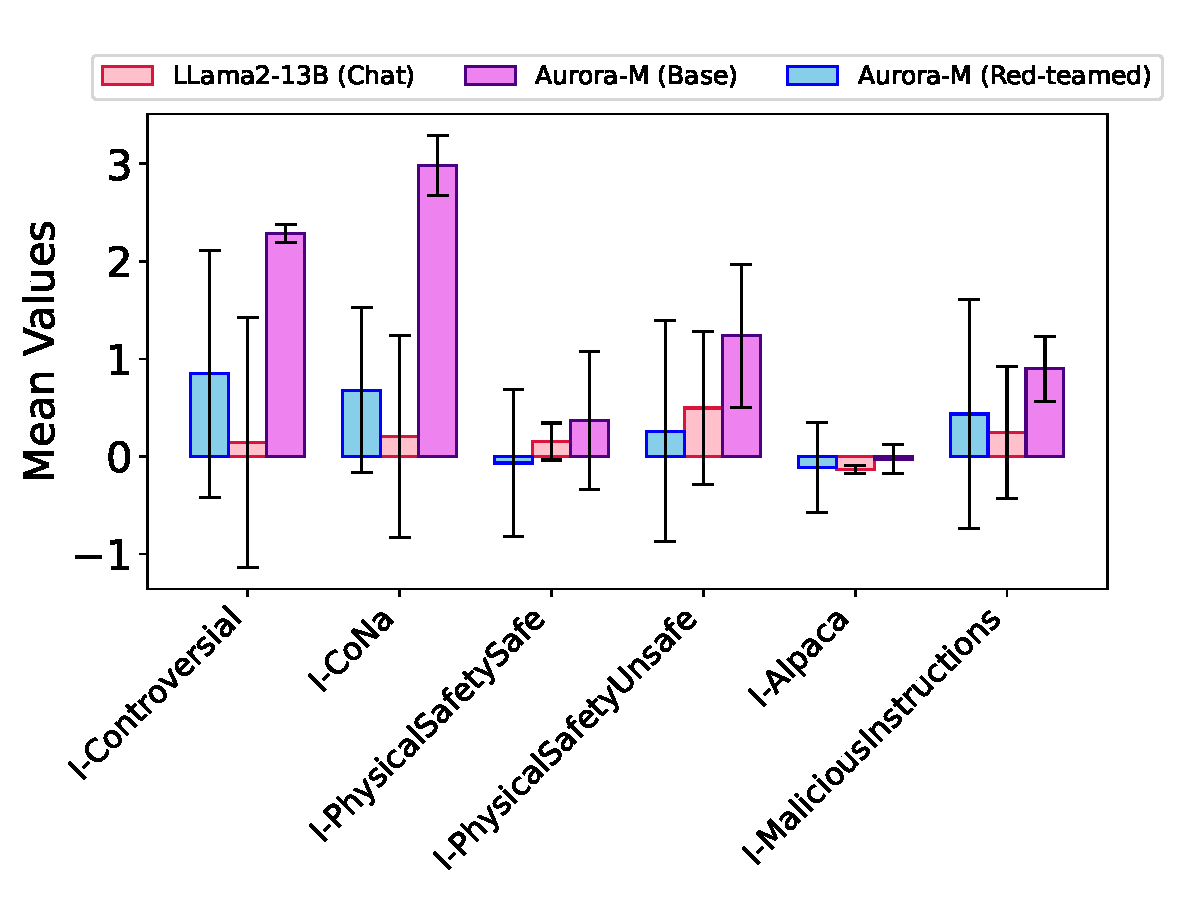
\includegraphics[width=\textwidth]{fig/harmfulnes_score.pdf}
        \caption{Harmfulness scores of our base model (pink) compared to its instruction-tuned version (blue). The lower the better.}
        \label{fig:safety-results}
    \end{subfigure}
    \hfill
    \begin{subfigure}{0.49\textwidth}
        \label{dangerous_qa}
        \centering
        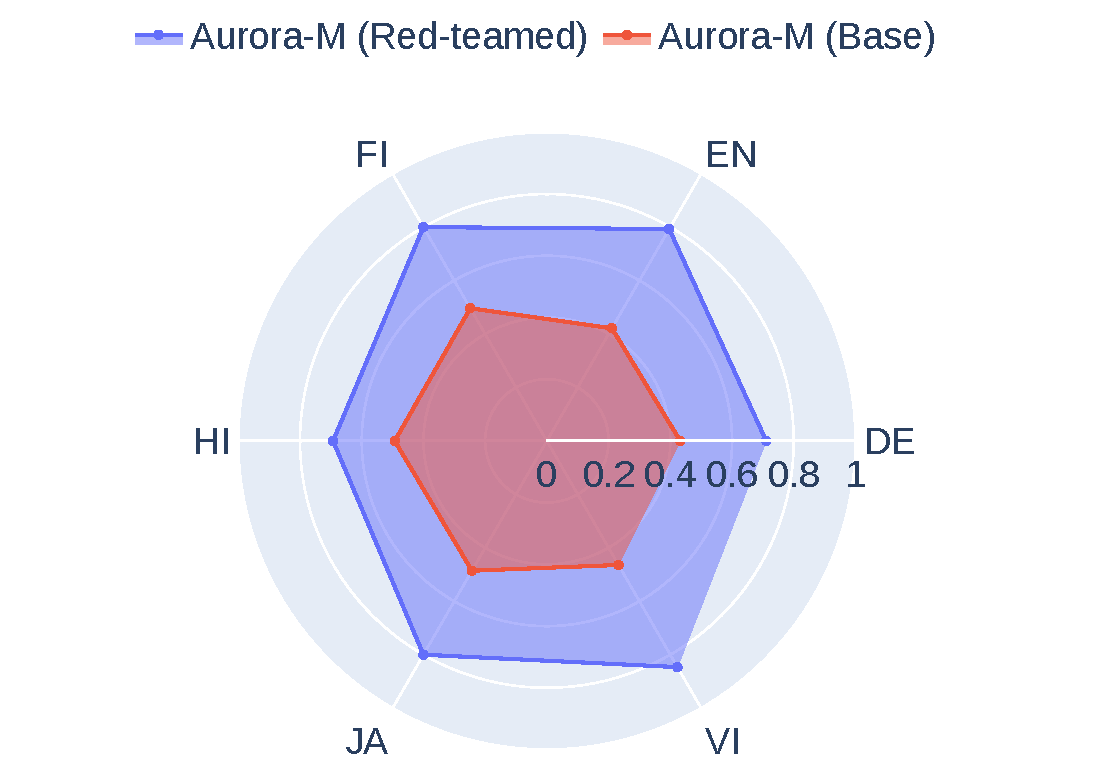
\includegraphics[width=\textwidth]{fig/bh_plot-8.pdf}
        \caption{CARP scores for the BH-readteamed model and the base model on the Biden-Harris Redteam Testset.}\label{fig:safety_bh}
    
        % \label{dangerous_qa}
        % \centering
        % 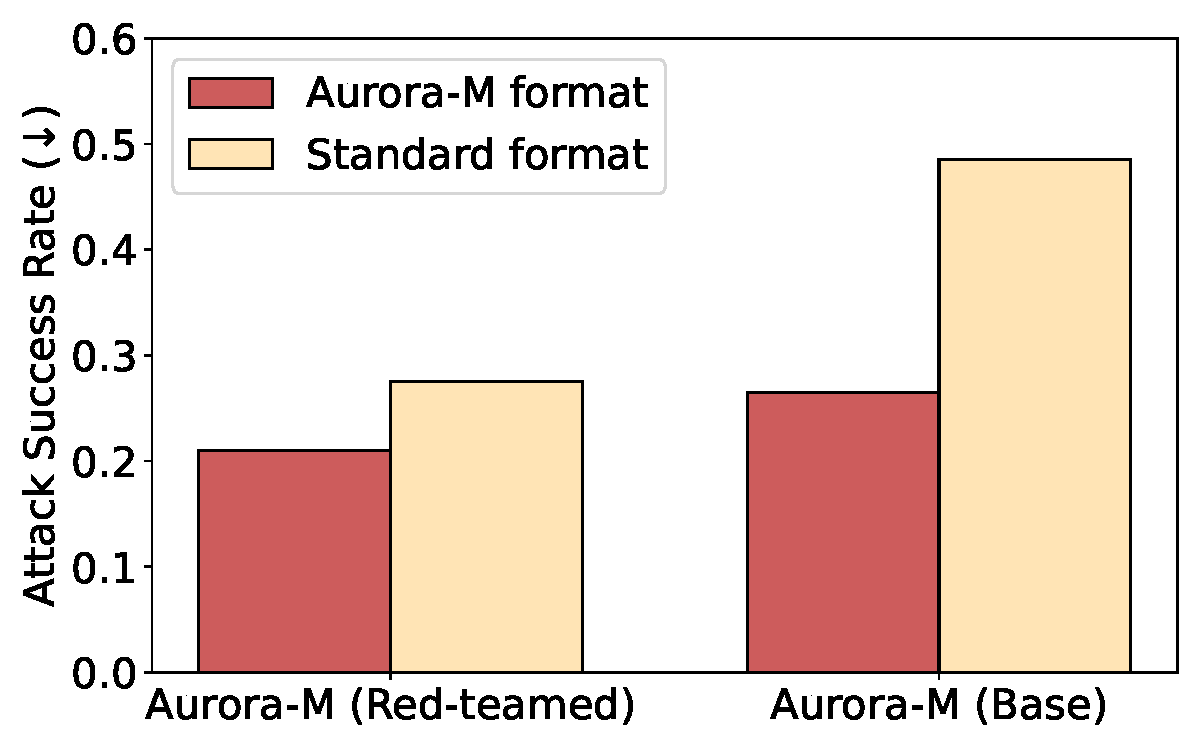
\includegraphics[width=\textwidth]{fig/asr.pdf}
        % \caption{ASR of DangerousQA queries on our base model (right) and its instruction-tuned version (left). The lower the better).}\label{fig:safety_dangerous}
    \end{subfigure}
    \caption{Overall safety results.}
    \label{fig:safety_results}
    \vspace{-0.3em}
\end{figure}


\subsection{Evaluation Results}
% @Yekun Chai

Figure~\ref{fig:overall} illustrates the superior performance of {\system} compared to its base model (\emph{i.e.}, \textsc{StarCoderPlus}) across an extensive range of code and multilingual benchmarks, underscoring the efficacy of {\system} across diverse fields and languages. We observe that \system\ can maintain performance on previously learned English and Code benchmarks while significantly outperforming on new language benchmarks. 
%for English, Hindi, Finnish and Vietnamese. These benchmarks encompass multiple categories including code generation (HumanEval, MBPP, HumanEvalFix, MultiPL-E), English language (OpenBookQA, TriviaQA, HelaSwag, SQuAD2.0, XWINO, GSM8K), Finnish language (FIN-bench), Japanese language (jp-stable\footnote{\url{https://github.com/Stability-AI/lm-evaluation-harness/tree/jp-stable}}, llm-jp-eval\footnote{\url{https://github.com/llm-jp/llm-jp-eval}}), Vietnamese language (ARC, HellaSwag, MMLU, TruthfulQA), and Hindi language (ARC, HellaSwag, MMLU, TruthfulQA). This consistent outperformance underscores the efficacy of {\system} across diverse fields and languages.



% \paragraph{Vietnamese.} For Vietnamese (Table~\ref{tab:merged-evaluation}) in the ARC, HellaSwag, and TruthfulQA tasks, and showing competitive performance in MMLU tasks. This is indicative of a robust cross-lingual transfer capability.

% \paragraph{Hindi.} In Hindi (Table~\ref{tab:merged-evaluation}) evaluations, \system\ also demonstrates an impressive ability to understand and generate responses, outperforming all other models.

\paragraph{Evaluation on Natural Languages.}

Tables~\ref{tab:japanese-evaluation},~\ref{tab:finish-evaluation},~\ref{tab:merged-evaluation},~\ref{tab:english-evaluation} demonstrate the respective performance on the targeted languages, showing that {\system} consistently outperforms the performance of its starting checkpoint, \textsc{StarCoderPlus}, and many other baselines, such as \textsc{Llama-2-7b}.  %Specifically, the results presented in Table~\ref{tab:japanese-evaluation},~\ref{tab:finish-evaluation},~\ref{tab:merged-evaluation},~\ref{tab:english-evaluation} demonstrate the efficacy of the model in handling tasks in Japanese (JA), Finnish (FI), Vietnamese (VI), Hindi (HI), and English (EN) respectively.


% @Taishi
% \paragraph{Japanese.} In Table \ref{tab:japanese-evaluation}, we observe that {\system} outperforms its predecessor, StarCoderPlus, across all tasks with the exception of SUM, where it remains competitive. This is indicative of a substantial gain in multi-task language understanding capabilities, particularly in multiple-choice, question-answering, and machine translation tasks for Japanese.




% \subsection{フィンランド語の評価}
% 表 \ref{tab:finish-evaluation} にフィンランド語の評価結果を示す. 

% \begin{table}[thb]
% \centering
% % \caption{フィンランド語の評価}
% \resizebox{0.44\textwidth}{!}{%
% \begin{tabular}{l | cccc}
% \toprule
% \textbf{Model} & \textbf{0-shot} & \textbf{1-shot} & \textbf{2-shot} & \textbf{3-shot} 
% \\ \midrule
% gpt3-finnish-8B & 42.66 & 46.53 & 47.96 & 48.41 \\
% gpt3-finnish-13B & 42.45 & 46.53 & 47.14 & 48.08 \\
% StarCoderBase & 37.07 & 42.65 & 42.11 & 44.43 \\
% StarCoderPlus & 34.85 & 43.97 & 44.05 & 46.49 \\
% Llama-2-7b-hf & 39.49 & 46.99 & 49.03 & 49.60 \\
% Llama-2-13b-hf & 45.69 & 55.70 & 56.93 & \textbf{57.50} \\
% {\system} & \textbf{51.80} & \textbf{56.11} & \textbf{57.77} & 57.48 \\
% \bottomrule
% \end{tabular}}
% \hspace{1mm}
% \resizebox{0.535\textwidth}{!}{%
% \begin{tabular}{l | cccc | c}
% \toprule
% \textbf{Model} & \textbf{ARC} & \textbf{HellaSwag} & \textbf{MMLU} & \textbf{TruthfulQA} & \textbf{Avg.} \\ 
%  & 0-shot & 0-shot & 0-shot & 0-shot &  \\ \midrule
% StarCoderBase & 22.14 & 29.74 & 27.11 & 44.84 & 30.96 \\
% StarCoderPlus & 24.27 & 32.67 & 27.35 & \textbf{45.49} & 32.45 \\
% bloom-7b1 & 24.87 & 37.97 & 25.65 & 44.77 & 33.32 \\
% Llama-2-13b-hf & 30.17 & 38.49 & \textbf{31.76} & 44.61 & 36.26 \\
% Llama-2-7b-hf & 25.64 & 35.20 & 27.95 & 45.15 & 33.49 \\
% VinaLlama-7b & 28.63 & 37.39 & 27.15 & 43.13 & 34.08 \\
% {\system} & \textbf{31.97} & \textbf{41.98} & 30.94 & 44.71 & \textbf{37.40} \\
%  \bottomrule
% \end{tabular}}
% \caption{Finnish (left) and Vietnamese (right) Evaluation.}
% \label{tab:vi-evaluation}
% \end{table}


% \paragraph{Finnish.} Table~\ref{tab:finish-evaluation} reveals the model's proficiency in a progressively challenging Finnish language evaluation setup, from 0-shot to 3-shot learning. Remarkably, {\system} not only surpasses StarCoderPlus but also exhibits superior performance compared to larger models like GPT3-Finnish-13B, particularly in few-shot scenarios, which highlights the model's effective learning from continual multilingual pre-training.


% \subsection{ベトナム語の評価}
% 表 \ref{tab:vi-evaluation} にベトナム語の評価結果を示す. 

% \begin{table}[thb]
% \centering
% % \caption{ベトナム語の評価}
% \resizebox{0.7\textwidth}{!}{%
% \begin{tabular}{l | cccc | c}
% \toprule
% \textbf{Model} & \textbf{ARC} & \textbf{HellaSwag} & \textbf{MMLU} & \textbf{TruthfulQA} & \textbf{Avg.} \\ 
%  & 0-shot & 0-shot & 0-shot & 0-shot &  \\ \midrule
% StarCoderBase & 22.14 & 29.74 & 27.11 & 44.84 & 30.96 \\
% StarCoderPlus & 24.27 & 32.67 & 27.35 & \textbf{45.49} & 32.45 \\
% Bloom-7b1 & 24.87 & 37.97 & 25.65 & 44.77 & 33.32 \\
% Llama-2-13b-hf & 30.17 & 38.49 & \textbf{31.76} & 44.61 & 36.26 \\
% Llama-2-7b-hf & 25.64 & 35.20 & 27.95 & 45.15 & 33.49 \\
% VinaLlama-7b & 28.63 & 37.39 & 27.15 & 43.13 & 34.08 \\
% {\system} & \textbf{31.97} & \textbf{41.98} & 30.94 & 44.71 & \textbf{37.40} \\
%  \bottomrule
% \end{tabular}}
% \caption{Vietnamese Evaluation.}
% \label{tab:vi-evaluation}
% \end{table}

% % \subsection{ヒンディー語の評価}
% % 表 \ref{tab:hi-evaluation}にヒンディー語の評価結果を示す. 
% \begin{table}[thb]
% \centering
% % \caption{ヒンディー語の評価}
% \resizebox{.7\textwidth}{!}{%
% \begin{tabular}{l| cccc |c}
% \toprule
% \textbf{Model} & \textbf{ARC} & \textbf{HellaSwag} & \textbf{MMLU} & \textbf{TruthfulQA} & \textbf{Avg.} \\ 
%  & 0-shot & 0-shot & 0-shot & 0-shot &  \\ \midrule
% StarCoderBase & 20.72 & 26.93 & 25.15 & 47.57 & 30.09 \\
% StarCoderPlus & 20.89 & 27.03 & 24.91 & \textbf{48.77} & 30.40 \\
% {\system} & \textbf{27.57} & \textbf{35.84} & \textbf{30.01} & 43.31 & \textbf{34.18} \\
% % bloom-7b1 & 0.2183 & 0.3164 & 0.2530 & 0.4439 & 0.3079 \\
% % Llama-2-13b-hf & 0.2098 & 0.2958 & 0.2619 & 0.4379 & 0.3014 \\
% % Llama-2-7b-hf & 0.2158 & 0.2819 & 0.2533 & 0.4637 & 0.3037 \\ 
% \bottomrule
% % vinallama-7b & 0.1875 & 0.2631 & 0.2412 & 0.3911 & 0.2707 \\ 
% \end{tabular}}
% \caption{Hindi Evaluation.}
% \label{tab:hi-evaluation}
% \end{table}



% \paragraph{English.} Table~\ref{tab:english-evaluation}, which presents the results of the English language evaluation, shows a clear trend where {\system} consistently outperforms StarCoderBase, and in several tasks, it outperforms StarCoderPlus as well. Notably, in the Winograd-style tasks (XWINO), {\system} establishes a new state-of-the-art, hinting at its nuanced understanding of the complexities of the English language.

% To summarize, the empirical evidence strongly suggests that {\system} is not only a successor to StarCoderPlus but also an advanced model that sets new benchmarks across various language understanding tasks. The performance leap is particularly evident in the multi-shot learning scenarios, which aligns with the intent to build a model that can quickly adapt to new languages and tasks with extended multilingual data.

\begin{table*}[!ht]
\centering
\resizebox{\textwidth}{!}{%
\begin{tabular}{l| ccc | ccc}
\toprule
\multicolumn{1}{c|}{\textbf{Model}} & \multicolumn{3}{c|}{\textbf{HumanEval}} & \multicolumn{3}{c}{\textbf{MBPP}} \\  
& Pass@1       & Pass@10      & Pass@100     & Pass@1       & Pass@10      & Pass@100     \\ \midrule
\textsc{StarCoderBase}~\citep{li2023starcoder} & \textbf{31.10} & \textbf{54.88} & \textbf{84.15} & 36.80 & \textbf{61.60} & \textbf{81.00} \\
\textsc{StarCoderPlus}~\citep{li2023starcoder} & 26.83 & 47.56 & 73.17 & 33.60 & 57.00 & 77.80 \\
\rowcolor{verylightgray}{\system} (Red-teamed) (Ours) & 29.27 & 49.39 & 81.71 & \textbf{38.60} & 61.00 & 78.00 \\
 \bottomrule
\end{tabular}}
\caption{HumanEval \& MBPP evaluation results.}
\label{tab:mbpp-human}
\end{table*}


\paragraph{Code Evaluation.}
Tables~\ref{tab:mbpp-human} and~\ref{tab:MultiPL-E} illustrate the proficiency of {\system} in code generation, demonstrating the possibility of continual pre-training from a code-centric checkpoint on multilingual data.
% 
In Table~\ref{tab:mbpp-human}, the HumanEval and MBPP evaluation benchmarks assess the model's ability to generate syntactically and semantically correct code snippets. {\system} exhibits competitive performance on the Pass@1 metric, which evaluates the model's ability to produce a correct answer on the first attempt.  In particular, {\system} consistently matches or outperforms StarCoderPlus, suggesting a significant improvement in code synthesis capabilities.
% 
In Appendix~\ref{app:code_extra}, we show results on additional code datasets and further analyze the behavior of our system by looking at the relationship between its performance and the number of training tokens across various languages and modalities.


\paragraph{Safety Evaluation}
In Figure \ref{fig:safety_results}, we provide the safety results comparing our base model against our Biden-Harris red-teamed model obtained by instruction-tuning the former on the dataset introduced in Section \ref{sec:safety}. For the Biden-Harris Redteam Testset evaluation, four volunteers reviewed both models' responses and scored them with -2 if harmful, 1 if not helpful but harmless, and 2 if both helpful and harmless. We term the percentage of the total score per category compared to its maximum possible score as the Continual Alignment Redteam Percentage ("CARP"). We can immediately appreciate the considerably lower harmfulness both on the existing benchmarks and on our own Biden-Harris red-team test set as evident by the CARP scores obtained by our red-teamed \system. \textit{We also note that even though our instruction set is predominantly in English, safety consistently improved not only in our target languages but also in languages we did not specifically focus on, such as German, thus showing strong indications of cross-lingual red-teaming effects}. Furthermore, as shown in Appendix~\ref{app:dangerous_qa}, the Attack Success Rate (ASR) on DangerousQA was also reduced. %Notably, from Figure \ref{fig:safety-results}, we observe that our model outperforms Llama 2 \citep{touvron2023llama} on three out of the six tested datasets, with Llama 2 being specifically designed to be aligned to human preferences for helpfulness and safety. Moreover, the aggregate harmless-helpful score using Biden-Harris Readteam Testset shows improvement across all our target languages. 

% \begin{figure}[!t]
% \begin{center}
% 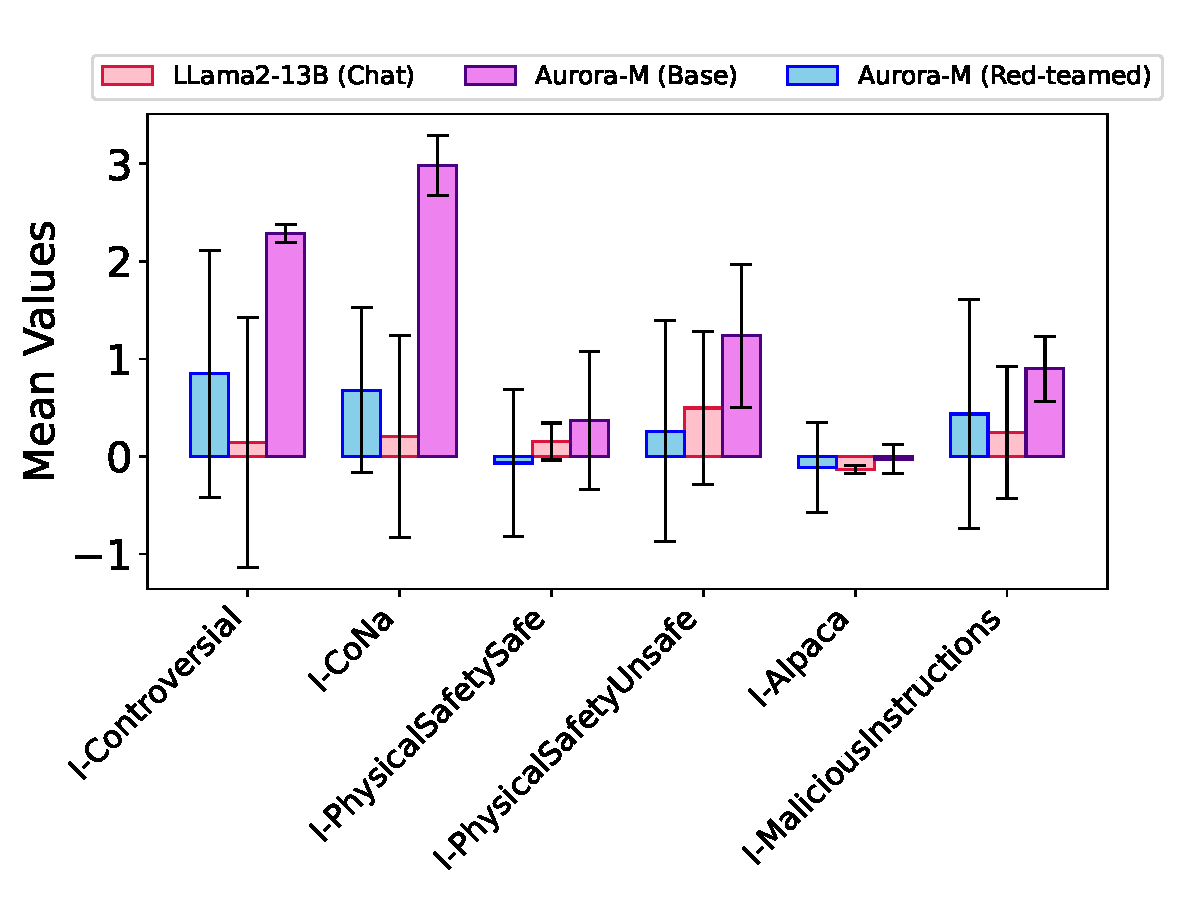
\includegraphics[width=0.8\textwidth]{fig/harmfulnes_score.pdf}
% \end{center}
% \caption{Safety results after instruction-tuning our model on the collected red teaming instruction-response pairs. }
% \label{fig:safety_results}
% \end{figure}



% \subsection{日本語の評価}
% 表 \ref{tab:japanese-evaluation} に日本語の評価結果を示す. 

% \begin{table*}[ht]
%     \centering
%         % \caption{日本語タスクにおける評価結果}
%         \caption{Japanese Evaluation}
%     \footnotesize
%     \begin{tabular}{l | r r r r r r r r | r}
%     \hline
%         \multicolumn{1}{c|}{Model} & \multicolumn{1}{c}{MC} & \multicolumn{2}{c}{QA} & \multicolumn{1}{c}{RC} & \multicolumn{1}{c}{SUM} & \multicolumn{1}{c}{MATH} & \multicolumn{2}{c}{MT (WMT20)} & \multicolumn{1}{|c}{Average}  \\ 
%         ~ & \multicolumn{1}{c}{JCom} & \multicolumn{1}{c}{JEMHop} & \multicolumn{1}{c}{NIILC} & \multicolumn{1}{c}{JSQuAD} & \multicolumn{1}{c}{XL-Sum} & \multicolumn{1}{c}{MGSM} & \multicolumn{1}{c}{En-Ja} & \multicolumn{1}{c|}{Ja-En} & ~ \\ 
%          & 4-shot & 4-shot & 4-shot & 4-shot & 1-shot & 4-shot & 4-shot & 4-shot & \\ \hline
%         StarCoderBase & 0.2976 & 0.4208 & 0.1794 & 0.7389 & 0.1396 & 0.0480 & 0.1513 & 0.0959 & 0.2589 \\
%         StarCoderPlus & 0.5022 & 0.4419 & 0.1772 & 0.7924 & 0.1687 & 0.0560 & 0.1458 & 0.1398 & 0.3030 \\
%         aurora-m-v0.1 (10k) & 0.4290 & 0.4527 & 0.3563 & 0.8485 & 0.0705 & 0.0360 & 0.2500 & 0.1666 & 0.3262 \\
%         aurora-m-v0.1 (20k) & 0.4549 & 0.4348 & 0.4046 & 0.8378 & 0.0655 & 0.0480 & 0.2573 & 0.1708 & 0.3342 \\
%         aurora-m-v0.1 (30k) & 0.2922 & 0.4143 & 0.3886 & 0.8550 & 0.0733 & 0.0440 & 0.2605 & 0.1849 & 0.3141 \\
%         aurora-m-v0.1 (40k) & 0.4111 & 0.4608 & 0.4274 & 0.8637 & 0.0779 & 0.0720 & 0.2662 & 0.1891 & 0.3460 \\
%         aurora-m-v0.1 (50k) & 0.4209 & 0.4690 & 0.4166 & 0.8675 & 0.0777 & 0.0480 & 0.2687 & 0.1890 & 0.3447 \\
%         aurora-m-v0.1 (60k) & 0.4468 & 0.4412 & 0.4558 & 0.8675 & 0.0838 & 0.0600 & 0.2712 & 0.1925 & 0.3524 \\
%         aurora-m-v0.1 (70k) & 0.4620 & 0.5019 & 0.4000 & 0.8703 & 0.0797 & 0.0640 & 0.2766 & 0.2002 & 0.3568 \\
%         aurora-m-v0.1 (80k) & 0.5040 & 0.4977 & 0.4599 & 0.8801 & 0.0873 & 0.0680 & 0.2782 & 0.2008 & 0.3720 \\
%         aurora-m-v0.1 (90k) & 0.5514 & 0.5064 & 0.4359 & 0.8816 & 0.0870 & 0.1000 & 0.2827 & 0.2069 & 0.3815 \\
%         aurora-m-v0.1 (95k) & 0.0188 & 0.0700 & 0.4419 & 0.8333 & 0.0910 & 0.2040 & 0.2702 & 0.1450 & 0.2593 \\
%         aurora-m-v0.1 (97.5k) & 0.3199 & 0.1772 & 0.4581 & 0.8269 & 0.0836 & 0.1840 & 0.2739 & 0.1692 & 0.3116 \\
%         aurora-m-v0.1 (100k) & 0.3557 & 0.2477 & 0.4987 & 0.8073 & 0.0872 & 0.1920 & 0.2696 & 0.0470 & 0.3132 \\
%         aurora-m-v0.1 (102k) & 0.3065 & 0.1883 & 0.4126 & 0.8450 & 0.0899 & 0.2040 & 0.2709 & 0.1053 & 0.3028 \\
%         {\system} & 0.4665 & 0.3573 & 0.5078 & 0.8706 & 0.0879 & 0.2120 & 0.2778 & 0.1722 & 0.3690 \\ 
%         % Llama-2-7b & 0.3852 & 0.4240 & 0.3410 & 0.7917 & 0.1905 & 0.0760 & 0.1783 & 0.1738 & 0.3201 \\
%         % Llama-2-13b & 0.6997 & 0.4415 & 0.4170 & 0.8533 & 0.2139 & 0.1320 & 0.2146 & 0.1982 & 0.3963 \\
%         \hline
%         \end{tabular}
%     \label{tab:japanese-evaluation}
% \end{table*}

% \subsection{英語の評価}
% 表 \ref{tab:english-evaluation} に英語の評価結果を示す. 
% \begin{table*}[ht]
%     \centering
%         % \caption{英語タスクにおける評価結果}
%         \caption{English Evaluation}
%     \footnotesize
%     \begin{tabular}{l | cccccc | c}
%     \hline
%     Model & OpenBookQA &  TriviaQA &  HellaSwag &  SQuAD2.0 &  XWINO &  GSM8K &  Average \\
%     & 8-shot & 8-shot & 8-shot & 8-shot & 8-shot & 8-shot & \\ \hline
%     StarCoderBase & 0.1960 & 0.0820 & 0.3757 & 0.2752 & 0.7351 & 0.0895 & 0.2922 \\
%     StarCoderPlus & 0.3480 & 0.5350 & 0.5806 & 0.3486 & 0.8925 & 0.1357 & 0.4734 \\
%     aurora-m-v0.1 (10k) & 0.3020 & 0.4290 & 0.5191 & 0.2527 & 0.8658 & 0.0978 & 0.4111 \\
%     aurora-m-v0.1 (20k) & 0.3060 & 0.4288 & 0.5162 & 0.2908 & 0.8645 & 0.0940 & 0.4167 \\
%     aurora-m-v0.1 (30k) & 0.3100 & 0.4313 & 0.5133 & 0.3025 & 0.8581 & 0.0978 & 0.4188 \\
%     aurora-m-v0.1 (40k) & 0.3020 & 0.4529 & 0.5154 & 0.2804 & 0.8753 & 0.1107 & 0.4228 \\
%     aurora-m-v0.1 (50k) & 0.2860 & 0.4583 & 0.5204 & 0.2946 & 0.8787 & 0.1122 & 0.4250 \\
%     aurora-m-v0.1 (60k) & 0.3100 & 0.4748 & 0.5197 & 0.2822 & 0.8710 & 0.1266 & 0.4307 \\
%     aurora-m-v0.1 (70k) & 0.3200 & 0.4974 & 0.5272 & 0.2944 & 0.8766 & 0.1327 & 0.4414 \\
%     aurora-m-v0.1 (80k) & 0.3220 & 0.5084 & 0.5317 & 0.2912 & 0.8843 & 0.1539 & 0.4486 \\
%     aurora-m-v0.1 (90k) & 0.3320 & 0.5201 & 0.5383 & 0.2978 & 0.8809 & 0.1630 & 0.4554 \\
%     aurora-m-v0.1 (95k) & 0.3520 & 0.4082 & 0.5406 & 0.4688 & 0.8847 & 0.0000 & 0.4424 \\
%     aurora-m-v0.1 (97.5k) & 0.3520 & 0.4427 & 0.5427 & 0.4828 & 0.8826 & 0.0000 & 0.4505 \\
%     aurora-m-v0.1 (100k) & 0.3560 & 0.4181 & 0.5418 & 0.4828 & 0.8839 & 0.0000 & 0.4471 \\
%     aurora-m-v0.1 (102k) & 0.3460 & 0.4758 & 0.5420 & 0.4712 & 0.8852 & 0.0000 & 0.4534 \\
%     {\system} & 0.3560 & 0.5186 & 0.5442 & 0.4703 & 0.8839 & 0.0000 & 0.4622 \\ \hline
%     \end{tabular}
%     \label{tab:english-evaluation}
% \end{table*}

% \subsection{フィンランド語の評価}
% 表 \ref{tab:finish-evaluation} にフィンランド語の評価結果を示す. 
% \begin{table}[h]
% \centering
% % \caption{フィンランド語の評価}
% \caption{Finnish Evaluation}
% \begin{tabular}{l | cccc}
% \hline
% Model & 0-shot & 1-shot & 2-shot & 3-shot 
% \\ \hline
% gpt3-finnish-8B & 0.4266 & 0.4653 & 0.4796 & 0.4841 \\
% gpt3-finnish-13B & 0.4245 & 0.4653 & 0.4714 & 0.4808 \\
% StarCoderBase & 0.3707 & 0.4265 & 0.4211 & 0.4443 \\
% StarCoderPlus & 0.3485 & 0.4397 & 0.4405 & 0.4649 \\
% aurora-m-v0.1 (10k) & 0.4647 & 0.5166 & 0.5234 & 0.5308 \\
% aurora-m-v0.1 (20k) & 0.4836 & 0.5223 & 0.5297 & 0.5386 \\
% aurora-m-v0.1 (30k) & 0.4572 & 0.5365 & 0.5470 & 0.5473 \\
% aurora-m-v0.1 (40k) & 0.4627 & 0.5343 & 0.5412 & 0.5430 \\
% aurora-m-v0.1 (50k) & 0.4667 & 0.5185 & 0.5370 & 0.5380 \\
% aurora-m-v0.1 (60k) & 0.4809 & 0.5442 & 0.5505 & 0.5657 \\
% aurora-m-v0.1 (70k) & 0.4591 & 0.5368 & 0.5408 & 0.5499 \\
% aurora-m-v0.1 (80k) & 0.4773 & 0.5428 & 0.5499 & 0.5645 \\
% aurora-m-v0.1 (90k) & 0.4647 & 0.5610 & 0.5633 & 0.5639 \\
% aurora-m-v0.1 (95k) & 0.4846 & 0.5640 & 0.5784 & 0.5893 \\
% aurora-m-v0.1 (97.5k) & 0.4877 & 0.5655 & 0.5702 & 0.5774 \\
% aurora-m-v0.1 (100k) & 0.4943 & 0.5584 & 0.5755 & 0.5742 \\
% aurora-m-v0.1 (102k) & 0.4914 & 0.5711 & 0.5809 & 0.5823 \\
% {\system} & 0.5180 & 0.5611 & 0.5777 & 0.5748 \\
% % Llama-2-7b-hf & 0.3949 & 0.4699 & 0.4903 & 0.4960 \\
% % Llama-2-13b-hf & 0.4569 & 0.5570 & 0.5693 & 0.5750 \\ 
% \hline
% \end{tabular}
% \label{tab:finish-evaluation}
% \end{table}

% \subsection{ベトナム語の評価}
% 表 \ref{tab:vi-evaluation} にベトナム語の評価結果を示す. 

% \begin{table}[h]
% \centering
% % \caption{ベトナム語の評価}
% \caption{Vietnamese Evaluation}
% \begin{tabular}{l | cccc | c}
% \hline
% Model & ARC & HellaSwag & MMLU & TruthfulQA & Average \\ 
%  & 0-shot & 0-shot & 0-shot & 0-shot &  \\ \hline
% StarCoderBase & 0.2214 & 0.2974 & 0.2711 & 0.4484 & 0.3096 \\
% StarCoderPlus & 0.2427 & 0.3267 & 0.2735 & 0.4549 & 0.3245 \\
% aurora-m-v0.1 (10k) & 0.2581 & 0.3725 & 0.2737 & 0.4107 & 0.3288 \\
% aurora-m-v0.1 (20k) & 0.2744 & 0.3804 & 0.2811 & 0.4372 & 0.3433 \\
% aurora-m-v0.1 (30k) & 0.2812 & 0.3815 & 0.2803 & 0.4153 & 0.3396 \\
% aurora-m-v0.1 (40k) & 0.2846 & 0.3883 & 0.2674 & 0.4088 & 0.3373 \\
% aurora-m-v0.1 (50k) & 0.2880 & 0.3901 & 0.2780 & 0.4345 & 0.3477 \\
% aurora-m-v0.1 (60k) & 0.3111 & 0.3964 & 0.2746 & 0.4347 & 0.3542 \\
% aurora-m-v0.1 (70k) & 0.2915 & 0.4031 & 0.2802 & 0.4202 & 0.3488 \\
% aurora-m-v0.1 (80k) & 0.3103 & 0.4040 & 0.2833 & 0.4281 & 0.3564 \\
% aurora-m-v0.1 (90k) & 0.3188 & 0.4062 & 0.2852 & 0.4307 & 0.3602 \\
% aurora-m-v0.1 (95k) & 0.3154 & 0.4153 & 0.3032 & 0.4299 & 0.3660 \\
% aurora-m-v0.1 (97.5k) & 0.3137 & 0.4170 & 0.3040 & 0.4434 & 0.3695 \\
% aurora-m-v0.1 (100k) & 0.3128 & 0.4179 & 0.3029 & 0.4380 & 0.3679 \\
% aurora-m-v0.1 (102k) & 0.3128 & 0.4164 & 0.3007 & 0.4482 & 0.3695 \\
% {\system} & 0.3197 & 0.4198 & 0.3094 & 0.4471 & 0.3740 \\
% % bloom-7b1 & 0.2487 & 0.3797 & 0.2565 & 0.4477 & 0.3332 \\
% % Llama-2-13b-hf & 0.3017 & 0.3849 & 0.3176 & 0.4461 & 0.3626 \\
% Llama-2-7b-hf & 0.2564 & 0.3520 & 0.2795 & 0.4515 & 0.3349 \\
% vinallama-7b & 0.2863 & 0.3739 & 0.2715 & 0.4313 & 0.3408 \\ \hline
% \end{tabular}
% \label{tab:vi-evaluation}
% \end{table}

% \subsection{ヒンディー語の評価}
% 表 \ref{tab:hi-evaluation}にヒンディー語の評価結果を示す. 
% \begin{table}[h]
% \centering
% % \caption{ヒンディー語の評価}
% \caption{Hindi Evaluation}
% \begin{tabular}{l| cccc |c}
% \hline
% Model & ARC & HellaSwag & MMLU & TruthfulQA & Average \\ 
%  & 0-shot & 0-shot & 0-shot & 0-shot &  \\ \hline
% StarCoderBase & 0.2072 & 0.2693 & 0.2515 & 0.4757 & 0.3009 \\
% StarCoderPlus & 0.2089 & 0.2703 & 0.2491 & 0.4877 & 0.3040 \\
% aurora-m-v0.1 (10k) & 0.2449 & 0.3217 & 0.2601 & 0.4158 & 0.3106 \\
% aurora-m-v0.1 (20k) & 0.2380 & 0.3311 & 0.2635 & 0.4260 & 0.3147 \\
% aurora-m-v0.1 (30k) & 0.2372 & 0.3363 & 0.2634 & 0.4239 & 0.3152 \\
% aurora-m-v0.1 (40k) & 0.2432 & 0.3406 & 0.2590 & 0.4024 & 0.3113 \\
% aurora-m-v0.1 (50k) & 0.2466 & 0.3448 & 0.2661 & 0.4276 & 0.3213 \\
% aurora-m-v0.1 (60k) & 0.2551 & 0.3456 & 0.2676 & 0.4166 & 0.3212 \\
% aurora-m-v0.1 (70k) & 0.2526 & 0.3489 & 0.2826 & 0.4075 & 0.3229 \\
% aurora-m-v0.1 (80k) & 0.2577 & 0.3499 & 0.2808 & 0.4162 & 0.3262 \\
% aurora-m-v0.1 (90k) & 0.2697 & 0.3562 & 0.2844 & 0.4097 & 0.3300 \\
% aurora-m-v0.1 (95k) & 0.2671 & 0.3596 & 0.2997 & 0.4342 & 0.3402 \\
% aurora-m-v0.1 (97.5k) & 0.2765 & 0.3600 & 0.3003 & 0.4307 & 0.3419 \\
% aurora-m-v0.1 (100k) & 0.2723 & 0.3608 & 0.2943 & 0.4224 & 0.3375 \\
% aurora-m-v0.1 (102k) & 0.2731 & 0.3599 & 0.3017 & 0.4330 & 0.3419 \\
% {\system} & 0.2757 & 0.3584 & 0.3001 & 0.4331 & 0.3418 \\
% % bloom-7b1 & 0.2183 & 0.3164 & 0.2530 & 0.4439 & 0.3079 \\
% % Llama-2-13b-hf & 0.2098 & 0.2958 & 0.2619 & 0.4379 & 0.3014 \\
% % Llama-2-7b-hf & 0.2158 & 0.2819 & 0.2533 & 0.4637 & 0.3037 \\ 
% \hline
% % vinallama-7b & 0.1875 & 0.2631 & 0.2412 & 0.3911 & 0.2707 \\ 
% \end{tabular}
% \label{tab:hi-evaluation}
% \end{table}

% \subsection{Code Evaluation}

% Table \ref{tag:mbpp-human} shows the results of humaneval and mbpp.

% Table \ref{tag:Multi-Lingual-HE} shows the results of Multi-Lingual Human-Eval.


% \begin{table}[h]
% \centering
% \caption{humaneval mbpp Evaluation}
% \begin{tabular}{l| ccc | ccc}
% \hline
% \multicolumn{1}{c|}{Model} & \multicolumn{3}{c|}{humaneval} & \multicolumn{3}{c}{mbpp} \\ \cline{2-7} 
% & pass@1       & pass@10      & pass@100     & pass@1       & pass@10      & pass@100     \\ \hline
% StarCoderBase & 0.3110 & 0.5488 & 0.8415 & 0.3680 & 0.6160 & 0.8100 \\
% StarCoderPlus & 0.2683 & 0.4756 & 0.7317 & 0.3360 & 0.5700 & 0.7780 \\
% aurora-m-v0.1 (10k) & 0.1951 & 0.4146 & 0.6341 & 0.2840 & 0.5200 & 0.6920 \\
% aurora-m-v0.1 (20k) & 0.2012 & 0.3537 & 0.6159 & 0.3020 & 0.5240 & 0.7200 \\
% aurora-m-v0.1 (30k) & 0.2256 & 0.4390 & 0.6646 & 0.2700 & 0.5120 & 0.7140 \\
% aurora-m-v0.1 (40k) & 0.2195 & 0.4024 & 0.6951 & 0.2980 & 0.5240 & 0.7260 \\
% aurora-m-v0.1 (50k) & 0.2012 & 0.3963 & 0.6890 & 0.2880 & 0.5300 & 0.7360 \\
% aurora-m-v0.1 (60k) & 0.2622 & 0.4268 & 0.7012 & 0.3040 & 0.5260 & 0.7320 \\
% aurora-m-v0.1 (70k) & 0.2744 & 0.4573 & 0.7500 & 0.3320 & 0.5800 & 0.7540 \\
% aurora-m-v0.1 (80k) & 0.2622 & 0.4878 & 0.7317 & 0.3440 & 0.5740 & 0.7460 \\
% aurora-m-v0.1 (90k) & 0.2927 & 0.4573 & 0.7744 & 0.3400 & 0.5680 & 0.7620 \\
% aurora-m-v0.1 (95k) & 0.2805 & 0.4756 & 0.7744 & 0.3660 & 0.5680 & 0.7860 \\
% aurora-m-v0.1 (97.5k) & 0.2683 & 0.5366 & 0.7866 & 0.3660 & 0.5980 & 0.7640 \\
% aurora-m-v0.1 (100k) & 0.2500 & 0.4939 & 0.7622 & 0.3800 & 0.5940 & 0.7660 \\
% aurora-m-v0.1 (102k) & 0.2805 & 0.5366 & 0.8110 & 0.3880 & 0.6120 & 0.7900 \\
% {\system} & 0.2927 & 0.4939 & 0.8171 & 0.3860 & 0.6100 & 0.7800 \\
%  \hline
% \end{tabular}
% \label{tag:mbpp-human}
% \end{table}

% \begin{table}[h]
% \centering
% \caption{Multi-Lingual HE}
% \begin{tabular}{l| ccc ccc | c}
% \hline
% Model & C++ & Java & PHP & TS & C\# & Bash & Average \\ \hline
% StarCoderBase & 0.2733 & 0.2595 & 0.2671 & 0.3333 & 0.2152 & 0.1076 & 0.2427 \\
% StarCoderPlus & 0.2671 & 0.2405 & 0.2671 & 0.2516 & 0.1772 & 0.0570 & 0.2101 \\
% aurora-m-v0.1 (10k) & 0.1739 & 0.1962 & 0.1118 & 0.2075 & 0.1456 & 0.0570 & 0.1487 \\
% aurora-m-v0.1 (20k) & 0.1988 & 0.1772 & 0.1304 & 0.2327 & 0.1013 & 0.0506 & 0.1485 \\
% aurora-m-v0.1 (30k) & 0.2050 & 0.2089 & 0.1366 & 0.2013 & 0.1266 & 0.0759 & 0.1591 \\
% aurora-m-v0.1 (40k) & 0.1739 & 0.2025 & 0.1304 & 0.1887 & 0.1392 & 0.0443 & 0.1465 \\
% aurora-m-v0.1 (50k) & 0.1615 & 0.2152 & 0.1118 & 0.2201 & 0.1139 & 0.0380 & 0.1434 \\
% aurora-m-v0.1 (60k) & 0.1801 & 0.1962 & 0.1491 & 0.2264 & 0.1139 & 0.0506 & 0.1527 \\
% aurora-m-v0.1 (70k) & 0.2236 & 0.2215 & 0.1429 & 0.2327 & 0.1266 & 0.0506 & 0.1663 \\
% aurora-m-v0.1 (80k) & 0.2298 & 0.2215 & 0.1615 & 0.2327 & 0.1582 & 0.0506 & 0.1757 \\
% aurora-m-v0.1 (90k) & 0.2050 & 0.2532 & 0.1677 & 0.2642 & 0.1456 & 0.0443 & 0.1800 \\
% aurora-m-v0.1 (95k) & 0.2422 & 0.2658 & 0.1491 & 0.2453 & 0.1266 & 0.0570 & 0.1810 \\
% aurora-m-v0.1 (97.5k) & 0.2112 & 0.2595 & 0.1801 & 0.2453 & 0.1646 & 0.0633 & 0.1873 \\
% aurora-m-v0.1 (100k) & 0.2236 & 0.2658 & 0.1801 & 0.2767 & 0.1392 & 0.0633 & 0.1915 \\
% aurora-m-v0.1 (102k) & 0.2236 & 0.2658 & 0.2112 & 0.2642 & 0.1709 & 0.0570 & 0.1988 \\
% {\system} & 0.2360 & 0.2595 & 0.2174 & 0.2516 & 0.1709 & 0.0696 & 0.2008 \\
% \hline
% \end{tabular}
% \label{tag:Multi-Lingual-HE}
% \end{table}





% \




% % \subsection{Initial experiments with BTM expert configurations and multilingual experts}
% % Following cBTM we wished to create experts that could be ensemble together to perform tasks on different provenances of data. However, we wished to lower the memory cost of running experts. Our hypothesis was that we could train and merge some layers of the model for each expert. Following [MEMIT]’s discussion on layer wise knowledge, we experimented with training the top portion of pythia 1b and 3b with different data mixtures.

% % We created data provenances following the pile data provenance and similar to the original BTM paper. We trained on each of: [list data]. We tested perplexity on individual model and merged models and found that the perplexity did not change much. We then trained 

% % We created a prototype model which merged experts [X,y,z] with a router trained on a fasttext text for each data domain. We found that the layerwise merging did create coherent text in the particular domain. We then trained a pythia 1b on Vietnamese text and attempted to merge the middle layers. However the results produced incoherent text. We concluded that this was because the original model did not have enough vietnamese knowledge in order to merge the new vietnamese expert. 







% We thus decided to perform a continued pretraining on our full expert dataset on startcoderplus. Moreover, we decided that LoRa based experts as described in [\_\_] would provide greater space savings than layer wise experts. Thus we trained [\_\_] lora experts on clustered data following [cBTM paper].


\subsection{Training Analysis}

% \paragraph{Performance Trends versus Training Token Compute}
% @yekun 
Figure \ref{fig:ana-code-en} and \ref{fig:ana-lg} show the relationship between the number of training tokens and the performance of the various models. This analysis aims to capture these trends for the code generation tasks such as HumanEval and MBPP, as well as for the English, Finnish, Hindi, Japanese, and Vietnamese language evaluations. We refer to Appendix~\ref{ap:ana} for detailed discussion.